\documentclass[a4paper]{article}
\usepackage{CJKutf8, indentfirst, graphicx}
\usepackage{listings, xcolor}
\lstset{basicstyle=\ttfamily,
  showstringspaces=false,
  commentstyle=\color{red},
  keywordstyle=\color{blue},
  language=sh
}
\begin{document}
\begin{CJK}{UTF8}{bsmi}
\title{Introduction to Computer Networks Lab1 Report}
\author{104021219 鄭余玄}
\date{}
\maketitle
\section{使用說明}
規格基本上是參考助教提供的規格書,細節列在實做過程中。而完整的使用方法和編譯方式都有使用 markdown 語法寫在 104021219\_readme.txt 檔案中。

\subsection{使用方法}
\begin{enumerate}
\item For socket server,
\begin{lstlisting}
./104021219_ser.exe <Port>
\end{lstlisting}
\item For socket client:
\begin{lstlisting}
./104021219_cli.exe <IPv4> <Port>
\end{lstlisting}
\end{enumerate}
註:缺少任何參數皆會顯示錯誤,並且不能執行。

\subsection{支援指令}
\begin{enumerate}
\item
\begin{lstlisting}
put <filename>
\end{lstlisting}

\item
\begin{lstlisting}
get <filename>
\end{lstlisting}

\item
\begin{lstlisting}
dir
\end{lstlisting}

\item
\begin{lstlisting}
rename <old filename> <new filename>
\end{lstlisting}
\end{enumerate}

\subsection{編譯環境}
\begin{enumerate}
\item Windows x64
\item Visual Studio 14.0
\item C++
\end{enumerate}

\section{實做過程}
不論 client 或是 server 程式,一開始都需要檢查 argc 和 argv 是否有足夠的參數可以啟動,此外我有做 port 範圍的驗證檢查,若有違反規則的,或是 Winsock 建立錯誤,則程式就不會啟動。

在 server 端的部份,因為所有操作都是在 ./upload 資料夾下,所以程式一啟動就直接創立並且切換到資料夾下,之後就可以開始監聽 client 端的封包,若是指令封包,則會顯示 client IP 執行指令後回傳的結果。此外,對於 socket 傳送或接收超過 MAX\_SIZE 大小的檔案,只需要使用 while 迴圈不斷接收封包,並且寫入或讀取到目前的檔案內容指標。

在 client 端的部份則是,每次讀取一行使用者輸入的指令,並且判斷屬於哪個規範的類型,之後再依據不同的操作,向 server 傳送或接收不同的檔案和切換資料夾。此外,透過計算 socket 傳輸檔案的 byte stream 大小,就可以知道檔案大小。

put 的實做方式是,先檢查 client 是否有此檔案,若無則拒絕操作。若有則再詢問 server 是否有此檔案名稱,若無則 server 回傳 WTF;如果有,則 server 回傳 LGTM,並且 client 詢問是否要覆蓋 server 端檔案。在檢查和確認完成之後,如果沒有要繼續 put 會送出 G8,若有則會送出 OK,並且直接開始傳送檔案。

get 的實做方式與 put 有點類似,先檢查 client 是否有此檔案,若有則詢問是否要覆蓋 client 端檔案,若不覆蓋則操作失敗。若有則再詢問 server 是否有檔案,若無則 server 回傳 WTF;如果有,則 server 回傳 LGTM,並且操作失敗。檢查完成之後,也是一樣直接開始傳輸檔案。

dir 的實做方式則是,在 server 端使用 system 函數下 dir 指令並且將資料流重新導向置 GBY.txt 這個暫存檔案,避免資料夾顯示內容過多,就可以透過類似 get 指令傳輸到 client  端之後就可以刪除。 client 讀取所有檔案內容後,經過部份內容處理後,就直接輸出結果,並且刪除 GBY.txt。因為 server 和 client 的 GBY.txt 是創立在 upload 和 download 資料夾外,所以不會有重複檔案名稱的問題。

rename 的實做方式是,server 會確認是否有舊檔案名稱,以及重新命名的檔案名稱是否有重複。若可以,就使用 system 函數下 ren 直接重新命名,並且回傳 G8。

\subsection{實驗}
在圖 \ref{fig:basic} 和圖 \ref{fig:error} 中,使用了703647 bytes 的純文字檔和 4137691 bytes 的 mp3 音檔來測試 socket 傳輸,而結果皆正確並且完全符合預期。

\begin{figure*}[h]
\centering{
    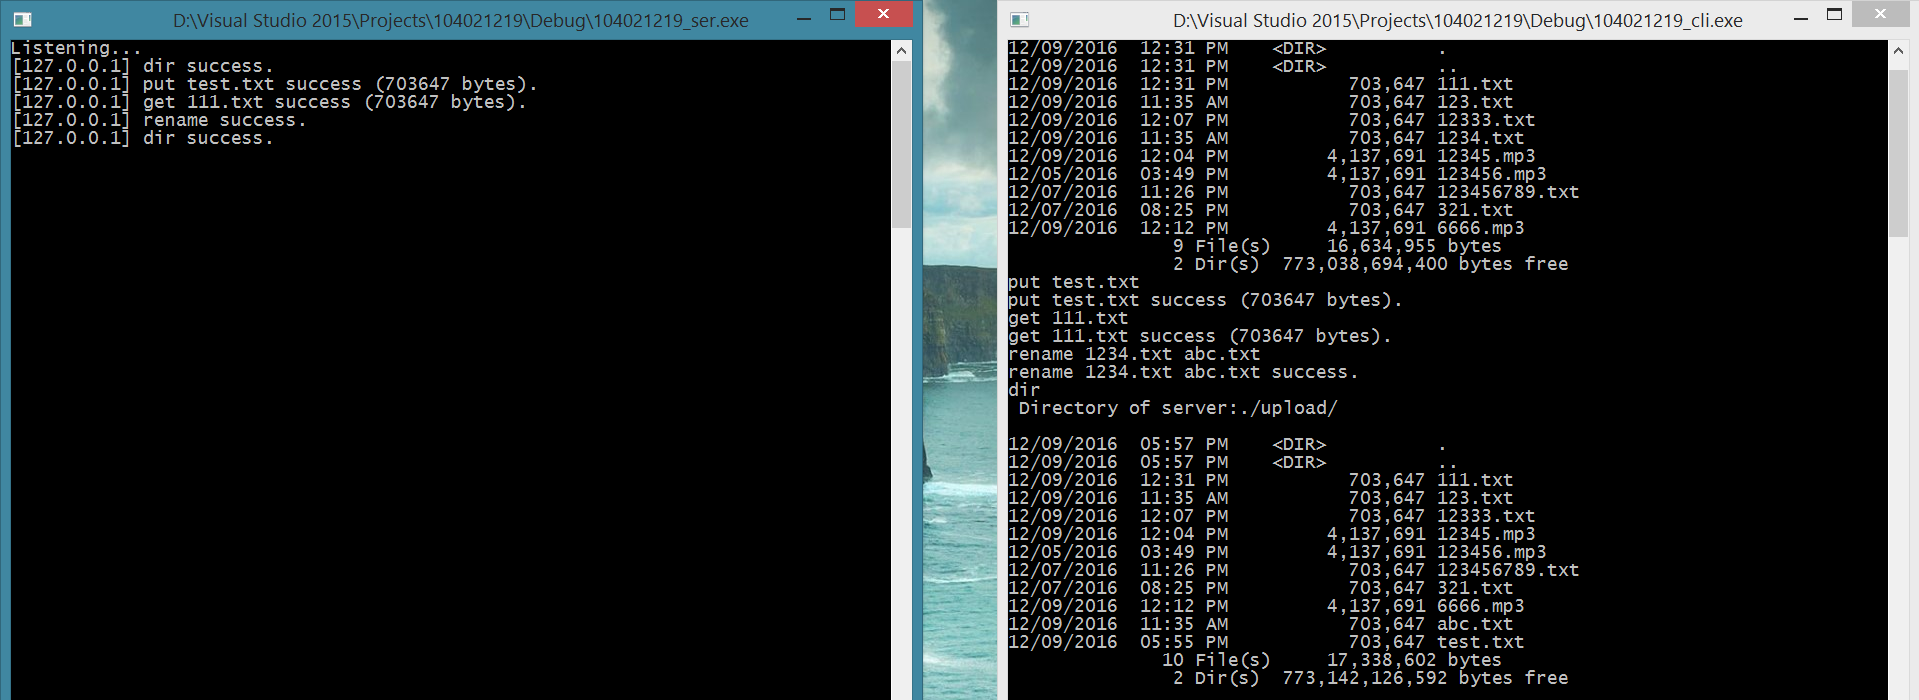
\includegraphics[width=1.2\textwidth]{basic}\label{fig:basic}
}
\caption{Basic}
\end{figure*}

\begin{figure*}[h]
\centering{
    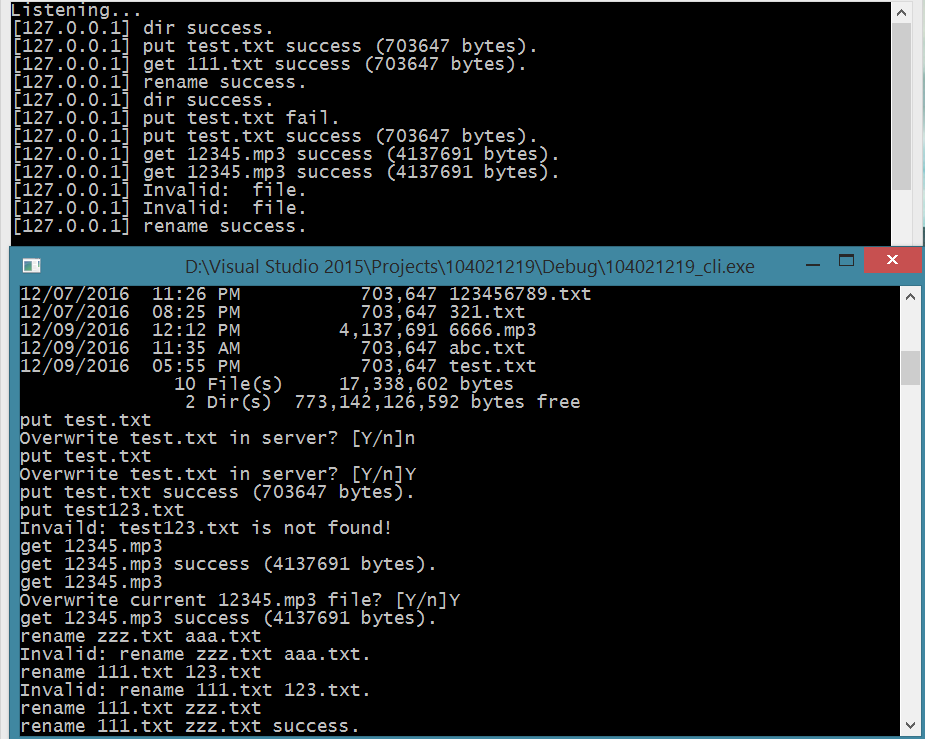
\includegraphics[width=.8\textwidth]{error}\label{fig:error}
}
\caption{Error Handling}
\end{figure*}

\section{學到的東西及遇到的困難}
因為我的開發環境是 Visual Studio 14.0,因此在引入 Winsock 時需要在程式碼中加上編譯參數:
\begin{lstlisting}[language=c++]
#pragma comment(lib, "Ws2_32.lib")
\end{lstlisting}

此外都是在複習 c++ 讀寫檔案的一些方法,基本上沒有遇到特別的困難。
\end{CJK}
\end{document}